\documentclass[main.tex]{subfiles}

\begin{document}

  \section{Superelliptic curves}\label{sec:se_curves}

  \subsection{Definition \& properties}

    \begin{defn}\label{def:se_curve}
%        A superelliptic curve over a field $K$ is a smooth cyclic branched covering of the projective line
%        $\cu \rightarrow \P^1_K$ of degree $m > 1$ such that $\text{char}(K)$ and $m$ are coprime.
    In this paper, a superelliptic curve $\cu$ over $\C$ is a smooth plane projective curve that has an affine model given by an equation of the form
   \begin{align}\label{eq:aff_model}
    \caff : \quad y^m = f(x) =  c_f \cdot \prod_{k=1}^n (x-x_k),
   \end{align}
   \end{defn}
   where $m > 1$ and $f \in \C[x]$ is separable of degree $n \ge 3$.
   Without loss of generality we may assume $c_f = 1$ (if not, apply the transformation $(x,y) \mapsto (x,\sqrt[m]{c_f}y)$).  \abstand
   Over $\C$ we identify the curve $\cu$ with the Riemann surface $\cu(\hat{\C})$ and denote by $\pr : \cu \rightarrow \P^1_{\C}$ the corresponding smooth cyclic branched covering of the projective line
   defined by the $x$-coordinate.

  There are $\delta = \gcd(m,n)$ points above infinity $P_{\infty}^{(1)},\dots,P_{\infty}^{(\delta)} \in \cu$, that behave differently depending on $m$ and $n$ (see \cite{CT1996}, \S 1 for details).
  Especially, $\infty \in \P^1_{\C}$ is a branch point for $\delta \ne m$. Thus, we introduce the set of finite branch points $X = \X$ as well as the set of all branch points
  \vspace{-0.3cm}
  \begin{align}\label{eq:branch_points}
         \hat{X} = \begin{cases}   X \cup \{ \infty \}, \quad \text{if}  m  \nmid  d,\\
         X,\quad \text{otherwise.}
     \end{cases}
  \end{align}
  The ramification indices at the branch points are given by $e_x = m$ for all $x \in X$ and $e_{\infty} = \frac{m}{\delta}$. Using the
  Riemann-Hurwitz formula, we obtain the genus of $\cu$ as
   \vspace{-0.3cm}
  \begin{align}\label{eq:genus}
    g = \frac{1}{2}( (m-1)(n-1) - \delta + 1).
  \end{align}




  \subsection{Complex roots and branches of the curve}\label{subsec:roots_branches}

  \subsubsection{The complex mth root}

  Working over the complex we encounter several multi-valued functions
  which we will briefly discuss here.  Closely related to superelliptic
  curves over $\C$ is the complex $m$-th root.
  Before specifying a branch it is a multi-valued function $y^m = x$
  that defines an $m$-sheeted Riemann surface, whose only branch points
  are at $x = 0,\infty$, and they're totally ramified.

  For $x\in\C$, it is natural and computationally convenient to use the
  \emph{principal branch} of the $m$-th root $\sqrt[m]x$ defined by
  \begin{equation}
      \label{eq:principal_mth_root}
      -\frac{π}m<\arg(\sqrt[m]x)\leq\frac{π}m
  \end{equation}
  which has a branch cut along the negative real axis $]\!-\infty,0]$.
  Crossing it in positive orientation corresponds to multiplication by
  the primitive $m$-th root of unity
  \begin{equation}
      \label{eq:zeta}
  \zeta = \zeta_m = e^{\frac{2\pi i }{m}}
  \end{equation}
  on the surface. In
  particular, the monodromy at $x=0$ is cyclic of order $m$.

  \subsubsection{The Riemann surface}

  As mentioned before, the equation $\caff : y^m = \prod_{k = 1}^n (x - x_k)$ defines an $m$-sheeted Riemann surface $\cu(\hat{\C})$. 
  Hence, there
  are $m$ possibilities to continue $y$ as an analytic function following a path in the $x$-plane. This is crucial for the intergration
  of differentials on $\cu$. Due to the cyclic structure of $\cu$, they are related in a convenient way:
  
  We call a \emph{branch of $\cu$} a function $y(x)$ such that
  $y(x)^m = f(x)$ for all $x \in \C$. At every $x$, the branches of $\cu$ only
  differ by a factor $\zeta^l$ for some $l \in \{0,\dots,l-1\}$. Thus, following a path, it is sufficient to know \emph{one} branch that is analytic in a suitable neighborhood. In the
  next paragraph, we will introduce locally analytic branches very explicitly.
  
  Similar to the complex $m$-th root, we can assume that crossing the branch cut at $x_k \in X$ in positive direction corresponds to multiplication by $\zeta$ on the surface. We
  obtain an ordering of the sheets relative to the analytic branches of $\cu$ by imposing that multiplication by $\zeta$ ( i.e. applying the map
  $(x,y(x)) \mapsto (x,\zeta y(x))$ ) corresponds to moving one sheet up on the surface.
  
  Consequently, the monodromy at every $x_k \in X$
  is equal and cyclic of order $m$ and thus, the monodromy group is isomorphic to the cyclic group $C_m$. This makes it possible to find explicit generators for the
  homology group $\homo$ without specifying a base point, as shown in \S \ref{m-subsec:cycles_homo}.
  
  
%   We call \emph{branch of $\cu$} a function $y(x)$ such that
%   $y(x)^m = f(x)$ for all $x \in \C$. At every $x$, the branches of $\cu$ only
%   differ by multiplication by a power of $\zeta$.
% 
%   In the case of superelliptic curves given
%   by an affine model $\caff : y^m = \prod_{k = 1}^d (x - x_k)$, indepently of
%   $d$ and $m$, every finite branch point $x_k$ is totally ramified, which means
%   the local monodromy is given by a cyclic permutation $\sigma_k \in S_m$.
% 
%   As we shall see below, we
%   will not impose a global ordering on the sheets of $\cu$. Instead we use
%   locally analytic branches $\yab$ (see \eqref{eq:def_yab}) and order them such that
%   moving one sheet up corresponds to the transformation $\yab \mapsto
%   \zeta\yab$. For us, encircling a branch point in positive orientation means
%   applying the local monodromy to the analytic branches of $\cu$, therefore we
%   can therefore assume that $\sigma_k = \sigma$ for $k = 1,\dots,d$.

  \subsubsection{Locally analytic branches}

  In order to integrate differential forms on $\cu$
% it is crucial to be able to follow an explicit analytic continuation of $y$ along a
  it is sufficient to be able to follow \emph{one} explicit analytic continuation of $y$ along a
  path joining two branch points $a, b \in X$.

  One could of course consider the \emph{principal branch} of the curve
  \begin{equation*}
      y(x) = \sqrt[m]{f(x)},
  \end{equation*}
  but this is not a good model to compute with: it has branch cuts
  wandering around the $x$-plane (see Figure \ref{fig:mth_root_principal}).
  
  A better option is to split the product as follows:
  assume that $a,b$ are the points $-1,1$. Then the function
  \begin{equation*}
      y(x) = \prod_{x_k\in X}\sqrt[m]{x-x_k}
  \end{equation*}
  has $n$ branch cuts parallel to the real line (see Figure \ref{fig:mth_root_product}).
  However, one of them lies exactly on the interval $[-1,1]$ we are interested in. We work around this
  by taking the branch cut towards $+\infty$ for each branch point $x_k$ with positive real part, writing
  \begin{equation*}
      y(x) = e^{\frac{iπr^+}m}\prod_{\Re(x_k)\leq0}\sqrt[m]{x-x_k} \prod_{\Re(x_k)>0}\sqrt[m]{x_k-x},
  \end{equation*}
  where $r^+$ is the number of points with positive real part.

  \todo (CN): Figure mth root signed missing? \\ difference between dashed and non-dashed lines? \\ remake pictures with tikz so they fit the style of the others?
  
  \begin{figure}[H]
      \begin{center}
          \subfloat[principal branch]{
          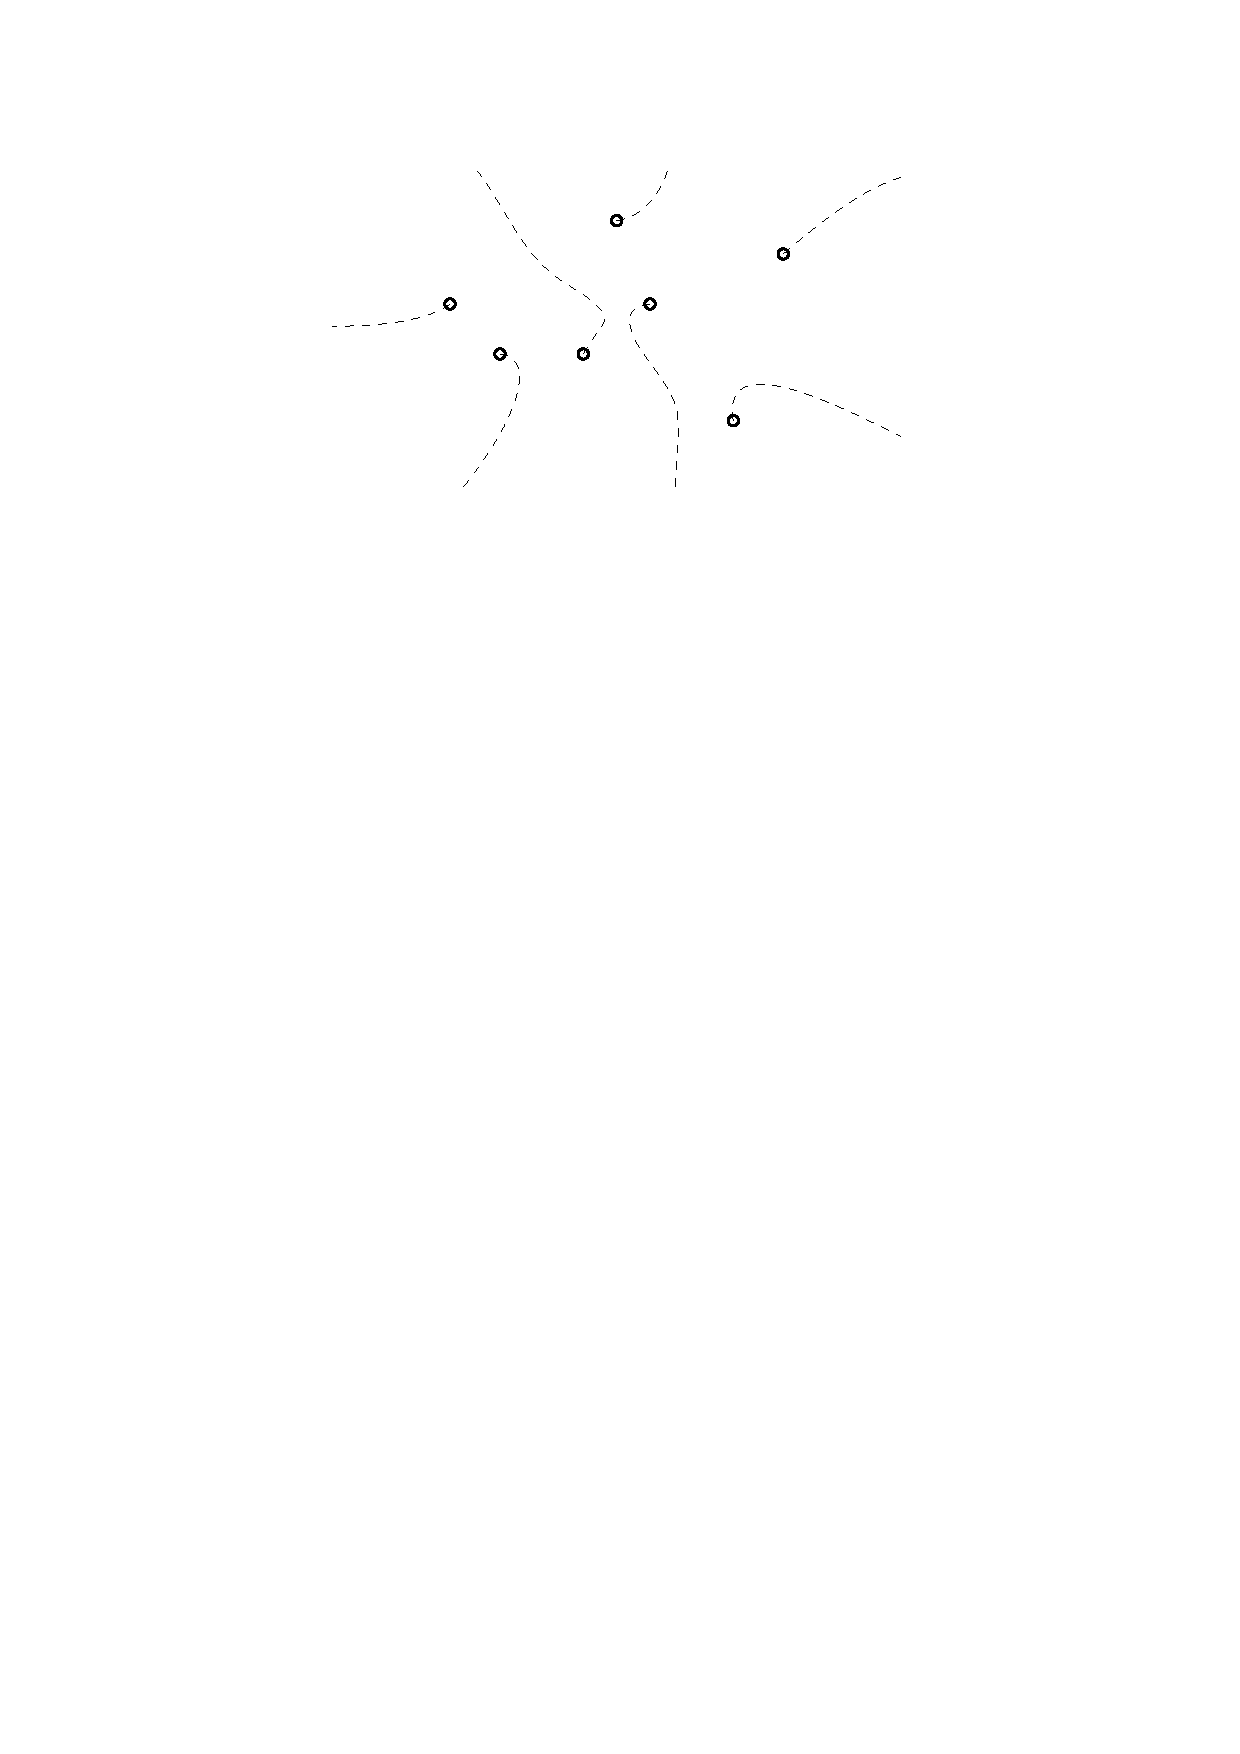
\includegraphics[width=.3\linewidth,page=1]{images/branch_cuts.pdf}
          \label{fig:mth_root_principal} }
          \subfloat[product]{ \includegraphics[width=.3\linewidth,page=2]{images/branch_cuts.pdf}\label{fig:mth_root_product} }
          \subfloat[$\yab$]{ \includegraphics[width=.3\linewidth,page=3]{images/branch_cuts.pdf}\label{fig:mth_root_signed} }
      \end{center}
      \caption{Branch cuts of different $m$-th roots.}
  \label{fig:mth_root_pol} \end{figure}

  In general we proceed the same way: For branch points $a,b \in X$ we consider the affine linear
  transformation
  \begin{equation}
      \label{def:uab}
      u_{a,b} : x \mapsto \frac{b-a}{2}\left(x+\frac{b+a}{b-a}\right),
  \end{equation}
  which maps $[-1,1]$ to the complex line segment $[a,b]$.
  
  We split the preimages of branch points into the following subsets
  \begin{equation*}
      \set{ u_{a,b}^{-1}(x) = \frac{2x-b-a}{b-a}, x\in X} = \set{-1,1} \cup U_{a,b}^+ \cup U_{a,b}^-,
  \end{equation*}
  where points in $U_{a,b}^+$ (resp. $U_{a,b}^-$) have strictly positive (resp. non-positive) real part.

  Then the product
  \begin{equation}
      \label{eq:ytab}
      \ytab(u) = \prod_{u_k\in U_{a,b}^-} \sqrt[m]{u-u_k}\prod_{u_k\in U_{a,b}^+}\sqrt[m]{u_k-u}
  \end{equation}
  is holomorphic on a neighborhood $ε_{a,b}$ of $[-1,1]$ which we can take as
  an ellipse \footnote{we will exhibit such a neighborhood in Section \ref{m-sub:gauss_chebychev_integration} \todo (CN) correct Reference? fig:ellipse exists 2 times?} 
  containing no point $u_k\in U_{a,b}^-\cup U_{a,b}^+$, while the term corresponding to $a,b$
  \begin{equation}
      \sqrt[m]{1-u^2}
  \end{equation}
  has two branch cuts $]-\infty,-1]$ and $[1,\infty[$, and is holomorphic on the complementary
  $\overline U_{a,b}$ of these cuts.
  
  We can now define the local branch
  \begin{equation}
      \label{eq:def_yab}
      \yab(x) =   C_{a,b} \yt_{a,b}( u_{a,b}^{-1}(x) ) \sqrt[m]{1 - u_{a,b}^{-1}(x)^2}
  \end{equation}
  where the constant
  \begin{equation}
      C_{a,b} = \left(\frac{b-a}{2}\right)^{\frac{n}{m}} e^{\frac{\pi i(1+\#U_{a,b}^+)}{m}}
  \end{equation}
  is chosen so that $\yab(x)^m = f(x)$.

  $y_{a,b}$ has $n$ branch cuts all parallel to $[a,b]$ in outward direction, and
  is holomorphic inside $]a,b[$ (see Figure \ref{fig:mth_root_signed}).

  More precisely, let $\vab = \uab(ε_{a,b}\cap \overline U_{a,b})$,
  so that $V_{a,b}$ is an ellipse shaped neighborhood of $]a,b[$ with two segments removed
  (see Figure \ref{m-fig:set_vab})
  on which the local branch $\yab$ is well defined and holomorphic.

  \begin{figure}[H] \begin{center} % Tikz File 'tikz_pic_14.tex'
% \documentclass{standalone}
% \usepackage{tikz}
% \usetikzlibrary{arrows}
% \usetikzlibrary{shapes.misc}
% \usetikzlibrary{decorations.markings}
% \tikzset{cross/.style={cross out, draw=black, minimum size=2*(#1-\pgflinewidth), inner sep=0pt, outer sep=0pt},cross/.default={1pt}}
% \tikzset{
%     halfarrow1/.style={postaction={decorate},
%         decoration={markings,mark=at position .5 with
%         {\arrow[line width=0.4mm]{>}}}} }
% \tikzset{
%     halfarrow2/.style={postaction={decorate},
%         decoration={markings,mark=at position .5 with
%         {\arrow[line width=0.4mm]{<}}}} }
% \begin{document}
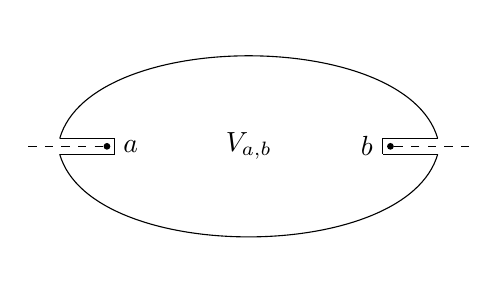
\begin{tikzpicture}

  \draw (-1.5,0) node {$a$};  \draw (1.5,0) node {$b$}; \draw (0,0) node {$V_{a,b}$};
  \filldraw [black] (-1.8,0) circle (1pt); \filldraw [black] (1.8,0) circle (1pt);
    \draw [dashed] (-2.8,0) -- (-1.8,0);   \draw [dashed] (2.8,0) -- (1.8,0);
    \draw (-2.4,0.1) .. controls (-2,1.5) and (2,1.5) .. (2.4,0.1);
    \draw (-2.4,-0.1) .. controls (-2,-1.5) and (2,-1.5) .. (2.4,-0.1);
    \draw (-2.4,-0.1) -- (-1.7,-0.1); \draw (2.4,-0.1) -- (1.7,-0.1);
    \draw (-2.4,0.1) -- (-1.7,0.1); \draw (2.4,0.1) -- (1.7,0.1);
    \draw (-1.7,0.1) -- (-1.7,-0.1); \draw (1.7,0.1) -- (1.7,-0.1);

\end{tikzpicture}


  \end{center} \caption{Holomorphic neighborhood of $\yab$.}
  \label{fig:set_vab} \end{figure}


  \begin{prop}\label{prop:yab}
      Let $a,b\in X$ be branch points such that $X\cap]a,b[=\varnothing$.
      Then, with the notations above, the functions
      $\ytab$ \eqref{eq:ytab} and $\yab$ \eqref{eq:def_yab}
      satisfy
     \begin{itemize}
         \item $\ytab$ is holomorphic and does not vanish on $ε_{a,b}$,
         \item $\yab(x)^m = f(x)$ for all $x\in\C$,
         \item $\yab(x) = C_{a,b} \ytab(\uab^{-1}(x)) \sqrt[m]{1-\uab^{-1}(x)^2}$ is holomorphic
         on $\vab$,
         \item $\yab(x),\zeta\yab(x),\dots,\zeta^{m-1}\yab(x)$ are the $m$ different analytic continuations of $y$ on $\vab$.
     \end{itemize}
     Moreover, we can assume that for $x \in \vab$ applying the map $(x,\yab(x)) \mapsto (x,\zeta^l\yab(x))$ corresponds to moving up $l \in \Z/m\Z$ sheets on the Riemann surface.
 \end{prop}
 



  \subsection{Cycles and homology}\label{subsec:cycles_homo}

   In this paragraph we present an explicit generating set of $\homo$ that is obtained by connecting the locally analytic branches $\yab$, as defined in \eqref{eq:def_yab},
   while also taking advantage of the superelliptic structure of our curve.
   For simplicity we will identify all cycles on $\cu$ with their classes in $\homo$.

   \begin{defn}\label{def:elem_cycle}
   Let $a, b \in X$ be branch points such that $X\cap]a,b[=\varnothing$, where  $[a,b]$ is the oriented line segment connecting $a$ and $b$.
   We define the corresponding \textit{elementary cycle}
   \begin{align}
    \cyab = \{  (x,\yab(x))  \mid  x \in [a,b]  \} \cup \{ (x,\zeta  \yab(x))  \mid  x \in [b,a]  \}
   \end{align}
   and, for $l \in \Z/m\Z$, its \textit{shifts}
   \begin{align}
    \cyab^{(l)} = \{  (x,\zeta^l \yab(x))  \mid  (x,y) \in \cyab  \}.
   \end{align}
    \end{defn}

   By our discussion in \S \ref{subsec:roots_branches}, the $\cyab^{(l)}$ are smooth oriented closed paths in $\pi_1(\cu)$ that are given as concatination of
   lifts of the line segment $[a,b]$ to $\cu$. \abstand
   In $\pi_1(\cu)$
   they are homotopic to cycles that encirlce  $a$ in negative and $b$ in positive orientation, once each.
   By the definition of $\yab$ the branch cuts at the end points are outward and parallel to $[a,b]$. Thus, we have the following useful visualizations of $\cyabl$ on $\cu$:
   \begin{figure}[H]
      \begin{center}
   % Tikz File 'tikz_pic_13.tex'
\begin{tikzpicture}
     \draw (-1.8,2) node {$a$};  \draw (1.8,2) node {$b$};
     \draw [densely dashed] (-3.0,3) -- (-1.8,3);  \draw [densely dashed] (1.8,3) -- (3.0,3); \draw (-1.8,3) circle (1.3pt); \draw (1.8,3) circle (1.3pt);
      \draw (-1.8,3) -- (1.8,3) [halfarrow2];
   \draw [densely dashed] (-3.0,1) -- (-1.8,1);  \draw [densely dashed] (1.8,1) -- (3.0,1); \draw (-1.8,1) circle (1.3pt); \draw (1.8,1) circle (1.3pt);
\draw (-1.8,1) -- (1.8,1) [halfarrow1];
      
      
      \draw (3.5,2) node {$\sim$};
      
           \draw (5.2,2) node {$a$};  \draw (8.8,2) node {$b$};
     \draw [densely dashed] (4.0,3) -- (5.2,3);  \draw [densely dashed] (8.8,3) -- (10,3); \draw (5.2,3) circle (1.3pt); \draw (8.8,3) circle (1.3pt);
     
\draw (4.5,3) .. controls (4.5,2.4) and (6,2.6) .. (7,3) [halfarrow2];
\draw (7,3) .. controls (8,3.4) and (9.5,3.6) .. (9.5,3) [halfarrow2];

   \draw [densely dashed] (4,1) -- (5.2,1);  \draw [densely dashed] (8.8,1) -- (10,1); \draw (5.2,1) circle (1.3pt); \draw (8.8,1) circle (1.3pt);
\draw (4.5,1) .. controls (4.5,1.6) and (6,1.4) .. (7,1) [halfarrow1];
\draw (7,1) .. controls (8,0.6) and (9.5,0.4) .. (9.5,1) [halfarrow1];
\end{tikzpicture}

      \end{center}
    \caption{Representations of a cycle $\cyabl$.}
    \label{fig:elem_cycle}
\end{figure}

  \bigskip

  As it turns out, we do not need all elementary cycles and their shifts to generate $\homo$, but only those that correspond to edges in a \emph{maximal spanning tree}, which is constructed
  as follows: \abstand
   Consider the complete graph on the set of finite branch points $G = (X,E')$, i.e.\ $E' = \{  (a,b)  \mid  a,b \in X \}$.
   Each edge $e = (a,b) \in E$ gets assigned a capacity $\tau_e$ that indicates the cost of numerical integration along the interval $[a,b]$. \abstand
   Here, the integration process ist most favourable
   between branch points that are far away from the others, that is, according to the
   numerical integration schemes that will be employed. \abstand
   We now apply a standard 'maximal-flow' algorithm from graph theory, based on a greedy approach, that results in a spanning tree $T = (X,E)$, where $E \subset E'$ contains the $d-1$ best edges
   for integration that connect all vertices without producing cycles.

   \bigskip

  For an edge $e = (a,b) \in E$, we denote by $\gamma_e^{(l)}$ the shifts of the corresponding elementary cycle $\cyab$.

  \begin{thm}\label{thm:gen_set}
   The cycles $\Gamma = \left\{  \gamma_{e}^{(l)}  \mid  0 \le l <m-1,  e \in E  \right\}$ generate $\homo$.
  \end{thm}
  \begin{proof}
  Denote by $\alpha_a \in \pi(\P^1 \setminus \hat{X})$ a closed path that encircles the branch point $a \in \hat{X}$ exactly once. Then,  due to the relation $1 = \prod_{a \in \hat{X}} \alpha_a$,
  $\pi_1(\P^1 \setminus \hat{X})$ is freely generateted by $\{ \alpha_a \}_{a \in X}$, i.e. in the case $\delta \ne m$ we can omit $\alpha_{\infty}$. \abstand
  Since our covering is cyclic, we have that $
  \pi_1(\cu \setminus \pr^{-1}(\hat{X})) \isom \ker(\pi_1(\P^1 \setminus \hat{X}) \overset{\Phi}{\To} \Aut(\cu \setminus \pr^{-1}(\hat{X})))$ where $\Aut(\cu \setminus \pr^{-1}(\hat{X})) \isom C_m
  \subset S_m$
  and $\Phi(\alpha_a)$ is cyclic of order $m$ for all $a \in X$. Hence, for every word $\alpha = \alpha_1^{s_1}\dots \alpha_n^{s_n} \in \pi_1(\P^1 \setminus \hat{X})$ we have that
  $\alpha \in \ker(\Phi) \eq \sum_{i=1}^n s_i \equiv 0 \bmod m$. \abstand
  We now claim that $\pi_1(\cu \setminus \pr^{-1}(\hat{X})) = \langle  \alpha_a^{-s} \alpha_b^{s},  \alpha_a^m   \mid  s \in \Z, a,b \in X  \rangle$
  and proof this by induction on $n$: For $\alpha = \alpha_1^{s_1}$ $m$ divides $s_1$ and therefore $\alpha$ is generated by $\alpha_1^m$. For $n > 1$ we write
  $\alpha = \alpha_1^{s_1}\dots \alpha_n^{s_n} = (\alpha_1^{s_1} \dots \alpha_{n-1}^{s_{n-1}+s_n})(\alpha_{n-1}^{-s_n}\alpha_n^{s_n})$. \abstand
  We obtain the fundamental group of $\cu$ as
  $\pi_1(\cu) \isom \pi_1(\cu \setminus \pr^{-1}(\hat{X})) / \langle  \alpha_a^{e_a}  \mid  a \in \hat{X}  \rangle$, which is generated by
  $\{  \alpha_a^{-s} \alpha_b^{s}  \mid  s \in \Z/m\Z,  a,b \in X  \}$. $(*)$ \abstand
  All branch points $a,b \in X$ are connected by a path $(a,v_1,\dots,v_t,b)$ in the spanning tree, so we can write $\alpha_a^{-s} \alpha_b^{s} = (\alpha_a^{-s}\alpha_{v_1}^{s})
  (\alpha_{v_1}^{-s}\alpha_{v_2}^{s})\dots(\alpha_{v_{t-1}}^{-s}\alpha_{v_t}^{s})(\alpha_{v_t}^{-s}\alpha_b^{s})$ and hence we have that
  $\{ \alpha_a^{-s} \alpha_b^{s}  \mid  s \in \Z/m\Z,  (a,b) \in E \}$ generates $\pi_1(\cu)$ and therefore $\homo$. \abstand
%     All that is left to see, is that for each edge $e = (a,b) \in E$ there exists a bijection $\varphi_e$ between
%   $\{  \gamma_e^{(l)}  \mid  l \in \Z/m\Z  \} \overset{\varphi_e}{\longleftrightarrow} \{  \alpha_a^{-s} \alpha_b^{s}  \mid  s \in \Z/m\Z  \}$: \abstand
  If we choose basepoints $p_0 \in \P^1 \setminus \hat{X}$ for $\pi_1(\P^1 \setminus \hat{X})$ and $P_0 \in \pr^{-1}(p_0)$ for $\pi_1(\cu \setminus \pr^{-1}(\hat{X}))$ and $\pi_1(\cu)$ respectively, then,
  depending on the choice of $P_0$, for all $e = (a,b) \in E$ there exists $l_0 \in \Z/m\Z$ such that $\gamma_e^{(l_0)}$ is homotopic to $\alpha_a^{-1} \alpha_b$ in $\pi_1(\cu,P_0)$.
   In $\homo$ we have that $\alpha_a^{-s}\alpha_b^{s} = ( \alpha_a^{-1}\alpha_b)^s$, so we obtain the other powers by concatenating
  the shifts $\prod_{l = 0}^{s-1} \gamma_e^{(l_0+l)} = (\alpha_a^{-1}\alpha_b)^s$.
  This implies $1 = \prod_{l = 0}^{m-1} \gamma_e^{(l_0+l)} = \prod_{l = 0}^{m-1} \gamma_e^{(l)}$ and
   $$\{  \alpha_a^{-s} \alpha_b^{s}  \mid  s \in \Z/m\Z  \} \subset  \langle  \gamma_e^{(l)} 
  \mid  0 \le l < m-1 \rangle$$ and therefore $\homo = \langle  \Gamma  \rangle$.
  \end{proof}

  \begin{rmk}
  \begin{itemize}
   \item[$\bullet$] For $\delta = 1$, we have that $\# \Gamma = (m-1)(n-1) = 2g$. Therefore, $C$ is a basis for $\homo$ in that case.
   \item[$\bullet$] In the case $\delta = m$, the point at infinity is not a branch point. Leaving out one finite branch point in the spanning tree results in only $n-2$ edges. Hence,
   $\# \Gamma = (m-1)(n-2) = 2g$ and $C$ is a basis for $\homo$.
   \item[$\bullet$] In step $(*)$ of the proof, filling in the points above infinity creates relations among
  these generators:
  $1 = (\prod_{a \in X} \alpha_a)^{k \cdot e_{\infty}}$, $k = 1,\dots,\delta$. This corresponds to the term $-\delta$ in the formula \eqref{m-eq:genus} for the genus of $\cu$. 
  \end{itemize}
  \end{rmk}



\subsection{Differential forms}\label{subsec:diff_forms}

    The computation of the period matrix and the Abel-Jacobi map requires a basis of $\hd$ as $\C$-vector space. In this section we provide a basis that only
   depends on $m$ and $n$ and is suitable for numerical integration. \abstand
    Among the meromorphic differentials
    \begin{align*}
 \WM = \left\{  \omega_{i,j}   \right\}_{\substack{1 \le i \le n-1, \\ 1 \le j \le m-1}} \quad \text{with} \quad \omega_{i,j} = \frac{ \dx^i}{i y^j},
  \end{align*}
  there are exactly $g$ that are holomorphic  and they can be found by imposing a simple combinatorial condition on $i$ and $j$.


   \bigskip

     \begin{prop}\label{prop:holom_diff}
 Let $\delta = \gcd(m,n)$. The following differentials form  a $\C$-basis of $\hd$:
 \begin{align}\label{eq:holm_diff}
   \W =  \left\{  \omega_{i,j} \in \WM  \mid  -mi + jn - \delta \ge 0  \right\}
 \end{align}
     \end{prop}
     \begin{proof}
      First we show that the differentials in $\W$ are holomorphic.
      Let $\w_{i,j} = x^{i-1}y^{-j} \dx \in \WM$. We write down the relevant divisors
      \begin{align*}
       \div(x) & = \sum_{k=1}^m \left(0,\zeta^k\sqrt[m]{f(0)}\right) - \frac{m}{\delta} \cdot \sum_{l = 1}^{\delta} P_{\infty}^{(l)}, \\
       \div(y) & = \sum_{k = 1}^n (x_k,0) - \frac{n}{\delta} \cdot \sum_{l = 1}^{\delta}  P_{\infty}^{(l)}, \\
       \div(\dx) & = (m-1)\sum_{k = 1}^n (x_k,0) - \left(\frac{m}{\delta} + 1\right)\cdot \sum_{l = 1}^{\delta}  P_{\infty}^{(l)}.
      \end{align*}
     Putting together the information, for $P \in \cu$ lying over $x_0 \in \P^1_{\C}$, we obtain
     \begin{align}\label{eq:diff_cases}
      v_P(\omega_{i,j}) & = (i-1) v_P(x) + v_P(\dx)  - j v_P(y) =
 \begin{cases}
  \ge 0 \hfill \text{if} \; x_0 \ne x_k,\infty, \\
  = m-1-j \ge 0 \quad \text{if} \; x_0 = x_k, \\
  = \frac{(-mi-\delta+jn)}{\delta} \hfill \text{if}\;  x_0 = \infty.
 \end{cases}
     \end{align}
     We conclude: $\omega_{i,j} \in \WM$ is holomorphic if and only if $\omega_{i,j} \in \W$. \abstand
     Since the differentials in $\W$ are clearly $\C$-linearly independent, it remains to show that
     there are enough of them, i.e. $\#\W = g$. \abstand
     Counting the elements in $\W$ corresponds to counting lattice points $(i,j) \in \Z^2$ in the trapezoid given by the faces
     \begin{align*}
 1 \le i \le n-1,\\
 1 \le j \le m-1, \\
 i \le \frac{n}{m}j - \frac{\delta}{m}.
     \end{align*}
      \begin{figure}[H]
      \begin{center}
   % Tikz File 'tikz_pic_7.tex'
%\documentclass{standalone}
% \usepackage{tikz}
\usetikzlibrary{arrows}
\usetikzlibrary{shapes.misc}
\usetikzlibrary{decorations.markings}
\tikzset{cross/.style={cross out, draw=black, minimum size=2*(#1-\pgflinewidth), inner sep=0pt, outer sep=0pt},cross/.default={1pt}}
\tikzset{
    halfarrow1/.style={postaction={decorate},
        decoration={markings,mark=at position .5 with
        {\arrow[line width=0.4mm]{>}}}} }
\tikzset{
    halfarrow2/.style={postaction={decorate},
        decoration={markings,mark=at position .5 with
        {\arrow[line width=0.4mm]{<}}}} }
%\begin{document}
\begin{tikzpicture}
%      \draw (-1.8,2) node {$a$};  \draw (1.8,2) node {$b$};
%      \draw (-2.5,3) -- (-1.8,3);  \draw (1.8,3) -- (2.5,3); \filldraw [gray] (-1.8,3) circle (2pt); \filldraw [gray] (1.8,3) circle (2pt);
% \draw (-2.3,3) .. controls (-0.9,2.5) and (-0.9,2.5) .. (0,3) [halfarrow2];
% \draw (0,3) .. controls (0.9,3.5) and (0.9,3.5) .. (2.3,3) [halfarrow2];
% 
%      
%    \draw (-2.5,1) -- (-1.8,1);  \draw (1.8,1) -- (2.5,1); \filldraw [gray] (-1.8,1) circle (2pt); \filldraw [gray] (1.8,1) circle (2pt);
% \draw (-2.3,1) .. controls (-0.9,1.5) and (-0.9,1.5) .. (0,1) [halfarrow1];
% \draw (0,1) .. controls (0.9,0.5) and (0.9,0.5) .. (2.3,1) [halfarrow1];

\draw (-0.7,0) -- (8,0) [->]; \draw (8.5,0) node {$j$};
\draw (0,-0.7) -- (0,4) [->]; \draw (0,4.5) node {$i$};
\draw (1,-0.05) -- (1,0.05); \draw (1,-0.4) node {$1$};
\draw (2,-0.05) -- (2,0.05); \draw (2,-0.4) node {$2$};
\draw (3,-0.05) -- (3,0.05); \draw (3,-0.4) node {$3$};
\draw (4,-0.05) -- (4,0.05); \draw (4,-0.4) node {$4$};
\draw (5,-0.05) -- (5,0.05); \draw (5,-0.4) node {$5$};
\draw (6,-0.05) -- (6,0.05); \draw (6,-0.4) node {$6$};
\draw (7,-0.05) -- (7,0.05); \draw (7,-0.4) node {$7$};
\draw (-0.05,1) -- (0.05,1); \draw (-0.4,1) node {$1$};
\draw (-0.05,2) -- (0.05,2); \draw (-0.4,2) node {$2$};
\draw (-0.05,3) -- (0.05,3); \draw (-0.4,3) node {$3$};
\draw[gray] (1,1) -- (1,3);
\draw[gray] (1,1) -- (7,1);
\draw[gray] (7,1) -- (7,3);
\draw[gray] (1,3) -- (7,3);
\draw[gray] (0,-0.5) -- (8,3.5);
%\filldraw (1,1) circle (1pt); \draw [fill=white] (1,1) circle[radius= 0.9pt];
\filldraw [gray] (1,1) circle (1pt);
\filldraw [gray] (1,2) circle (1pt);
\filldraw [gray] (1,3) circle (1pt);
\filldraw [gray] (2,1) circle (1pt);
\filldraw [gray] (2,2) circle (1pt);
\filldraw [gray] (2,3) circle (1pt);
\filldraw (3,1) circle (1pt);
\filldraw [gray] (3,2) circle (1pt);
\filldraw [gray] (3,3) circle (1pt);
\filldraw (4,1) circle (1pt);
\filldraw [gray] (4,2) circle (1pt);
\filldraw [gray] (4,3) circle (1pt);
\filldraw (5,1) circle (1pt);
\filldraw (5,2) circle (1pt);
\filldraw [gray] (5,3) circle (1pt);
\filldraw (6,1) circle (1pt);
\filldraw (6,2) circle (1pt);
\filldraw [gray] (6,3) circle (1pt);
\filldraw (7,1) circle (1pt);
\filldraw (7,2) circle (1pt);
\filldraw (7,3) circle (1pt);
\end{tikzpicture}
%\end{document}

      \end{center}
    \caption{The points below the line correspond to holomorphic differentials. Illustraded is the case $n=4,m=8$, and thus $g = 8$.}
    \label{fig:holom_diff}
\end{figure}
     Carefully analyzing the situation at the vertices of the trapezoid, we find the following formula that counts the points.
     \begin{align}\label{eq:r_j}
 \#\W & = \sum_{j = 1}^{m-1} \floor*{\frac{n}{m}j - \frac{\delta}{m}} = \sum_{j = 1}^{m-1} \frac{nj-\delta-r_j}{m} =
  \frac{n}{m} \sum_{j=1}^{m-1} j - \frac{m-1}{m}\delta - \frac{1}{m} \sum_{j=1}^{m-1} r_j,
     \end{align}
      where $r_j := nj - \delta  \bmod m$. \abstand
      We claim that
      \begin{align}\label{eq:r_j2}
       \sum_{j=1}^{m-1} r_j = \frac{1}{2}(m^2 - (\delta+2)m + 2\delta).
      \end{align}
      In order to show this, let $l := \frac{m}{\delta}$. First we note that $r_j = r_{j+l}$:
      $$r_{j+l} = n(j+l) - \delta  \bmod m = nj + \frac{n}{\delta}m - \delta  \bmod m =  nj - \delta  \bmod m =  r_j$$
      and hence
      \begin{align}\label{eq:r_j3}
       \sum_{j=1}^{m-1} r_j = \delta \cdot \sum_{j=1}^{l} r_j - r_m = \delta \cdot \sum_{j=1}^{l} r_j - (-\delta + m).
      \end{align}
      Furthermore, $r_j$ can be written as multiple of $\delta$:
      $$r_j = \delta \left(\frac{n}{\delta}j - 1\right)  \bmod m.$$
      From $\gcd(\frac{n}{\delta},l) = 1$ we conclude $\left\{  \frac{n}{\delta}j - 1  \bmod l  \mid  1 \le j \le l  \right\} = \{  0,\dots,l-1  \}$.
      Therefore,
      \begin{align}\label{eq:r_j4}
       \sum_{j = 1}^l r_j = \sum_{j = 0}^{l-1} \delta j = \delta \cdot \frac{l(l-1)}{2}
      \end{align}
      and thus (\ref{eq:r_j3}) and (\ref{eq:r_j4}) imply
      $$\sum_{j=1}^{m-1} r_j = \delta \cdot \sum_{j=1}^{l} r_j + \delta - m = \delta^2 \cdot \frac{l(l-1)}{2} + \delta - m = \frac{1}{2}(m^2 - (\delta+2)m + 2\delta).$$
      Plugging (\ref{eq:r_j2}) into (\ref{eq:r_j}) yields
      \begin{align*}
 \#\W & = \frac{n}{m}\frac{m(m-1)}{2} - \frac{m-1}{m}\delta - \frac{m^2 - (\delta+2)m + 2\delta}{2m} \\
        & = \frac{n(m-1)}{2} - \delta  - \frac{m}{2} + \frac{\delta}{2} + 1 =  \frac{n(m-1) - (m-1) - \delta + 1}{2} \\
        & = \frac{1}{2}((n-1)(m-1)-\delta+1) = g.
      \end{align*}
     \end{proof}
     \begin{rmk}
      Note that from \eqref{eq:diff_cases} it follows that the meromorphic differentials in $\WM$ are homolorphic at every finite place.
     \end{rmk}






\biblio
\end{document}
